\documentclass[main.tex]{subfiles}
\begin{document}

To create the FSM model based on the identified states and transitions from the previous chapter, the Graphwalker Studio was used, a straightforward tool for setting up models with a drag-and-drop interface. After organizing the model visually, it can be exported to JSON format and manually edited to define inputs and outputs for each transition. The final result is the FSM model shown below.
\begin{figure}[H]
    \centering
    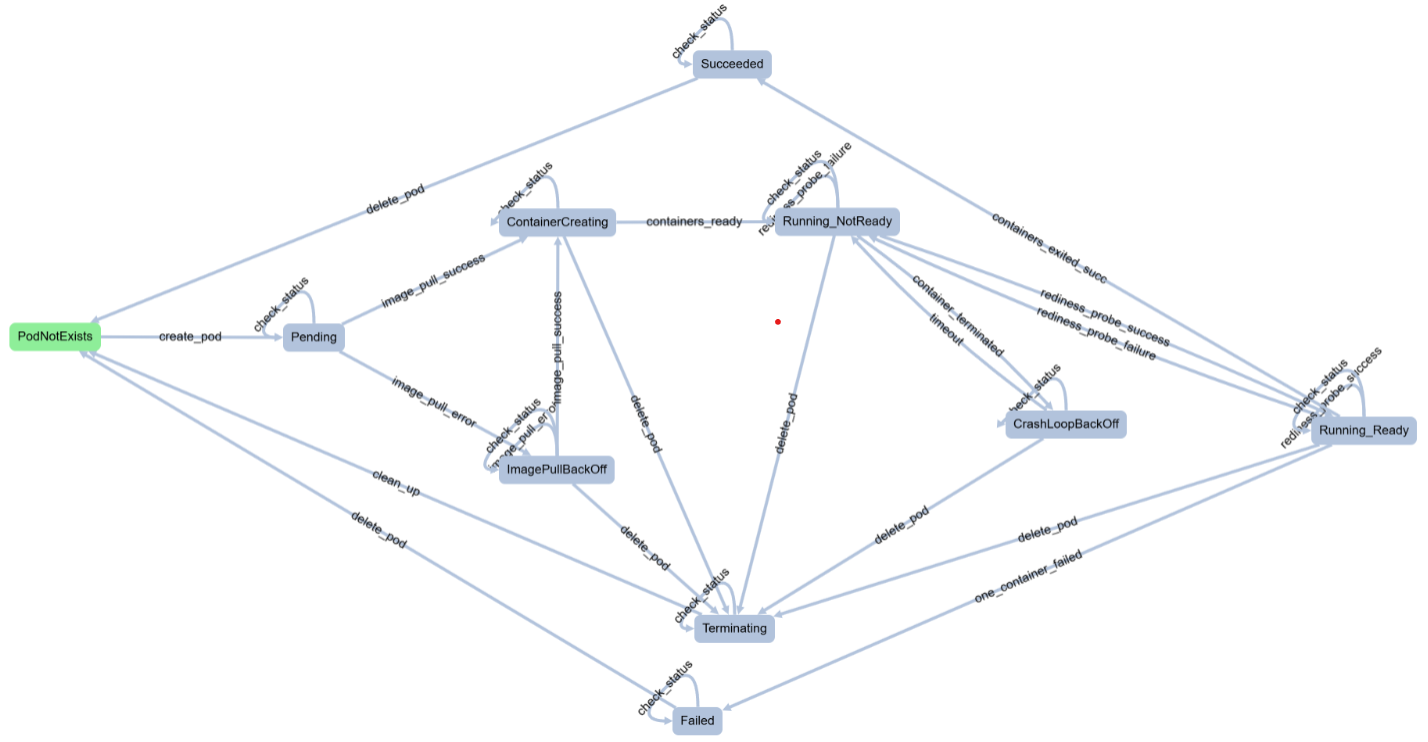
\includegraphics[width=\textwidth]{k8s_fsm_model.png}
    \caption{FSM model}
    \label{fig:fsm_model}
\end{figure}

The following figure is the extended version of the model, made by the MTR transition tour test generation algorithm with \texttt{--graphviz} flag. It also contains the input and output symbols too.
\begin{figure}[H]
    \centering
    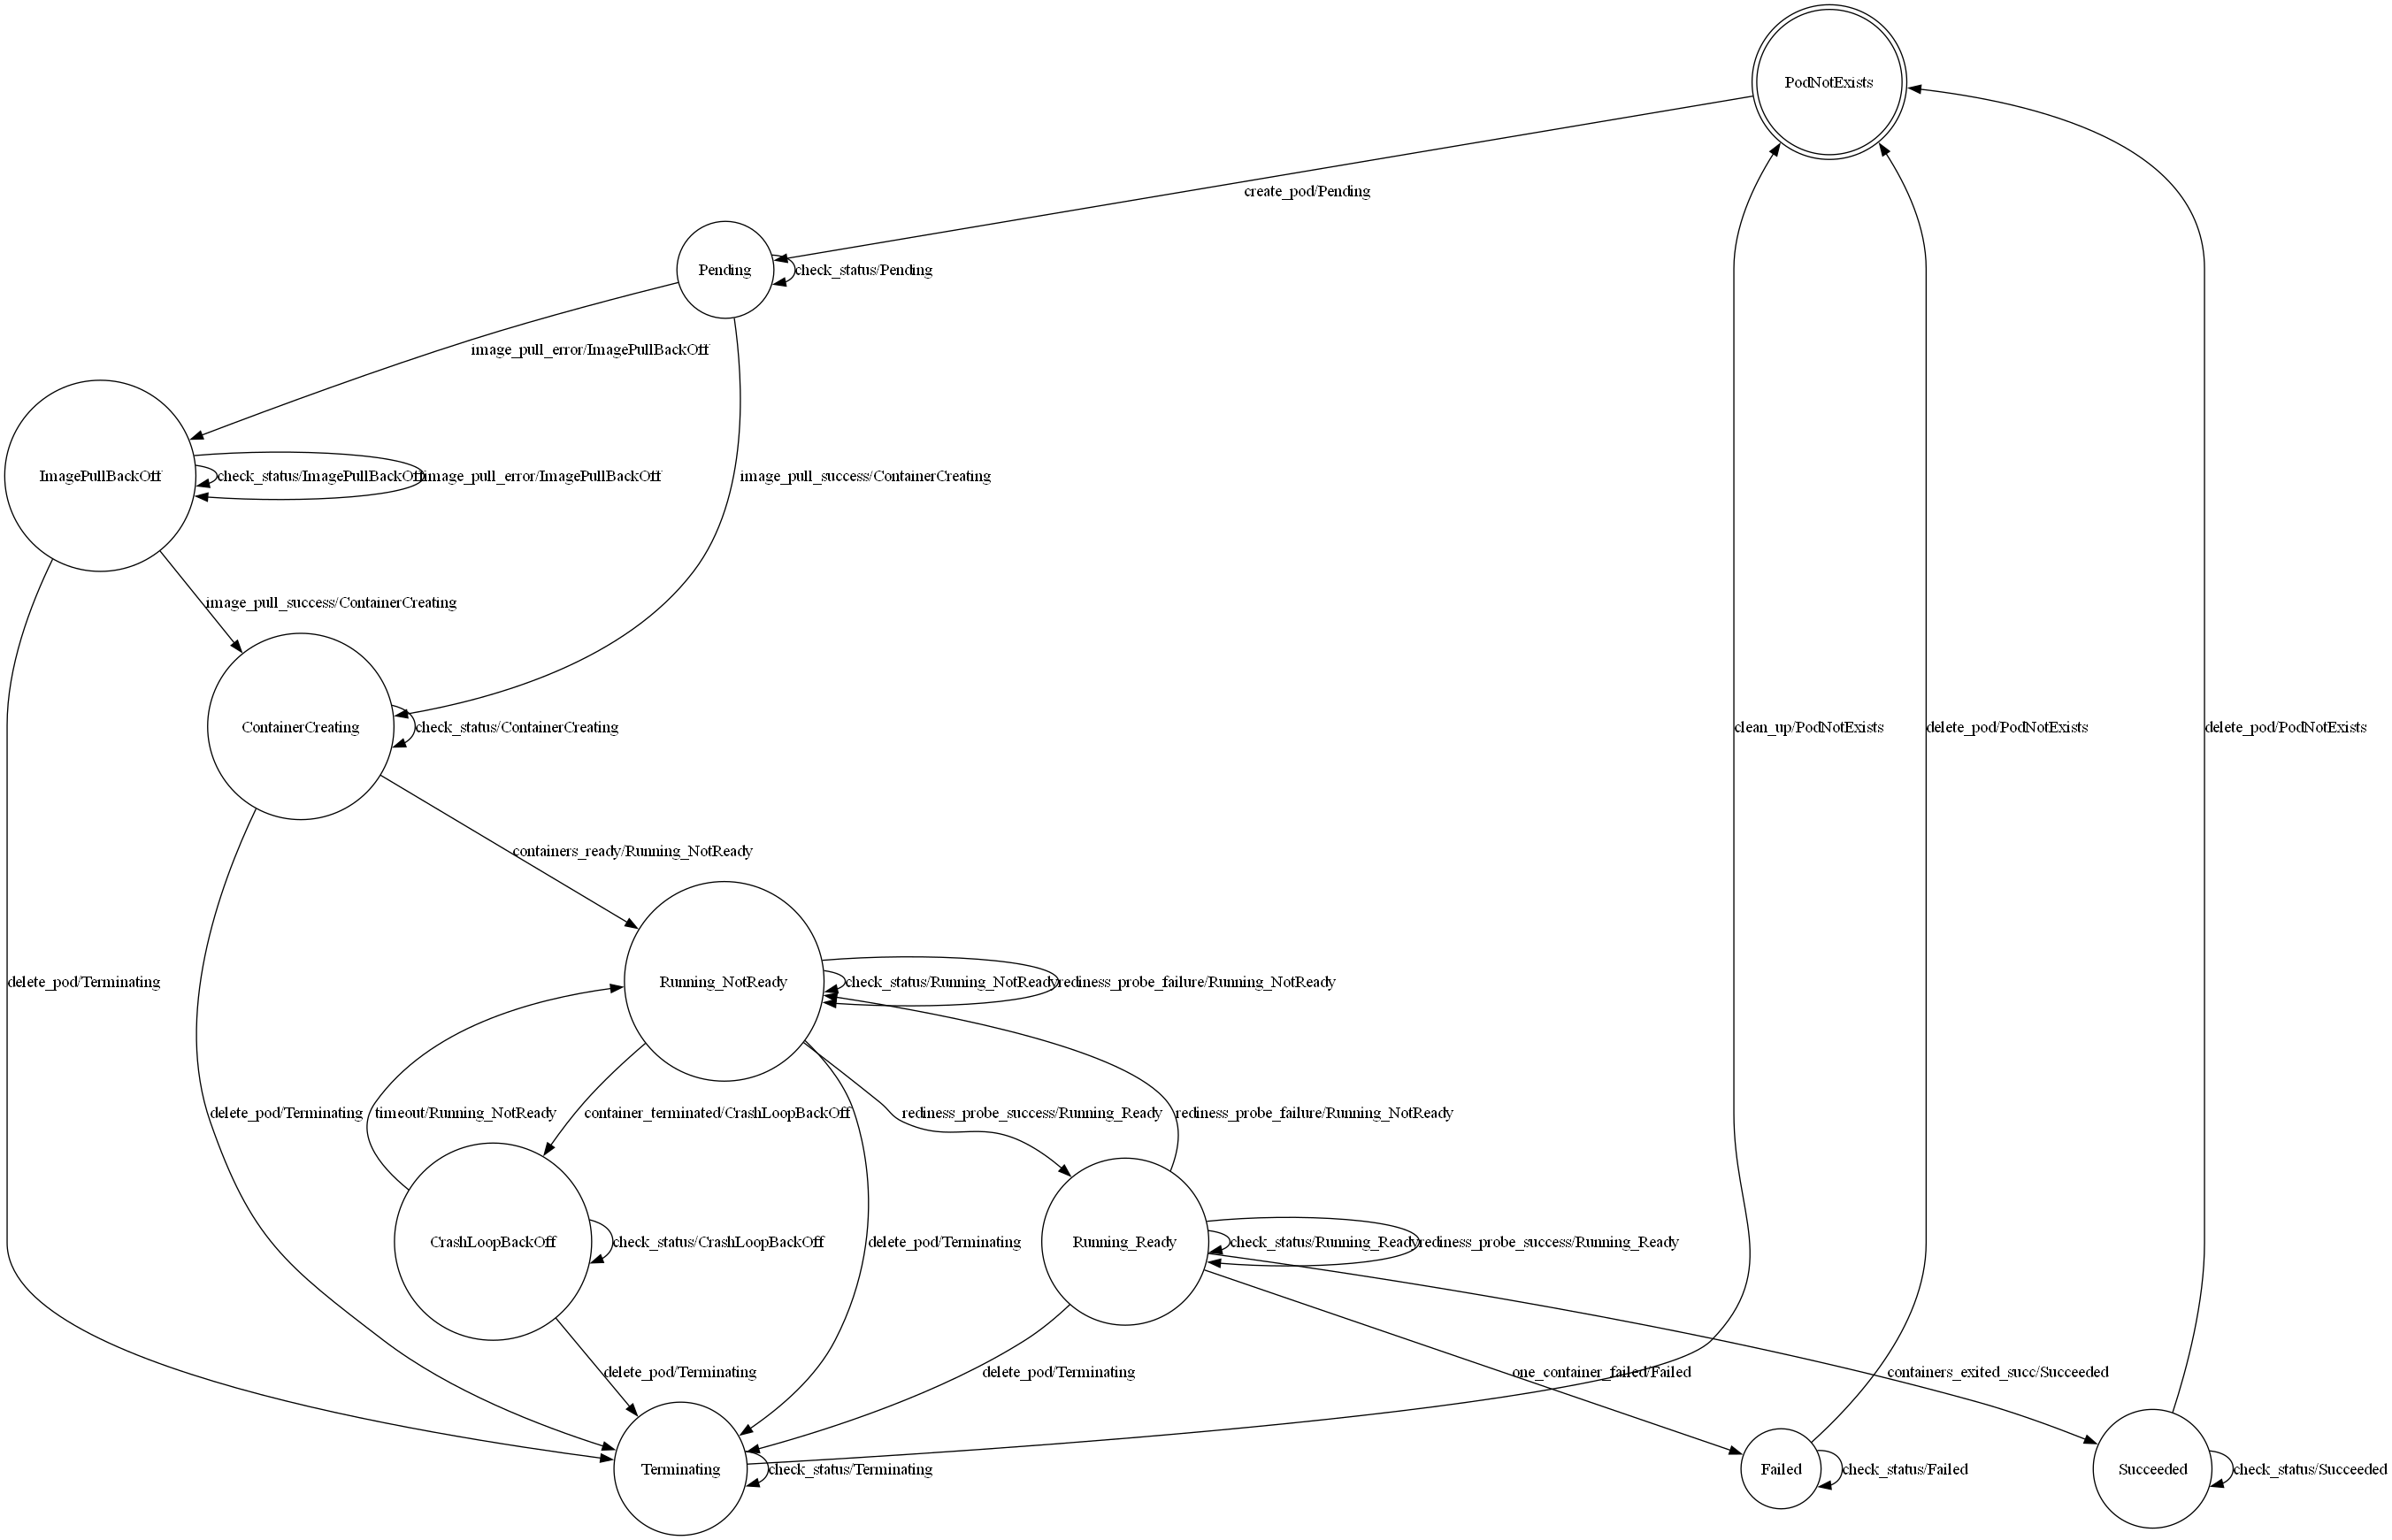
\includegraphics[width=\textwidth]{graphviz_image.png}
    \caption{Grapviz result}
    \label{fig:grapviz}

\end{figure}

\end{document}